% Pre-ambulo
\documentclass[a4paper, 12pt]{abnt}

\usepackage[brazil]{babel}
\usepackage[utf8]{inputenc}
\usepackage[T1]{fontenc}
\usepackage{dsfont}
\usepackage{amssymb,amsmath}
\usepackage{multirow}
\usepackage[alf]{abntcite}
\usepackage[pdftex]{color, graphicx}
\usepackage{colortbl}
\usepackage{url}
\usepackage{abnt-alf}
\usepackage{abntcite}
\usepackage{algorithm}
\usepackage{algorithmic}
\usepackage{tikz}
\usepackage{booktabs}
\usetikzlibrary{positioning, fit, arrows.meta, backgrounds}
%\usepackage{alg}
%\usepackage{hyperref}
\usepackage{listings}     
\usepackage{lstautogobble}  % Fix relative indenting
\usepackage{color}          % Code coloring
\usepackage{zi4}            % Nice font

\definecolor{bluekeywords}{rgb}{0.13, 0.13, 1}
\definecolor{greencomments}{rgb}{0, 0.5, 0}
\definecolor{redstrings}{rgb}{0.9, 0, 0}
\definecolor{graynumbers}{rgb}{0.5, 0.5, 0.5}

\usepackage{listings}
\lstset{
    autogobble,
    columns=fullflexible,
    showspaces=false,
    showtabs=false,
    breaklines=true,
    showstringspaces=false,
    breakatwhitespace=true,
    escapeinside={(*@}{@*)},
    commentstyle=\color{greencomments},
    keywordstyle=\color{bluekeywords},
    stringstyle=\color{redstrings},
    numberstyle=\color{graynumbers},
    basicstyle=\ttfamily\footnotesize,
    frame=l,
    framesep=12pt,
    xleftmargin=12pt,
    tabsize=4,
    captionpos=b
}

\renewcommand{\arraystretch}{1.5}

% Útil!
\newcommand{\tccTitle}{Geração de prosódia para o português brasileiro em sistemas \emph{text-to-speech}}
\newcommand{\tccTitleEn}{Prosody generation for Brazilian Portuguese in text-to-speech systems}
% Redefinicao de instrucoes
\floatname{algorithm}{Algoritmo}
\renewcommand{\algorithmicrequire}{\textbf{Entrada:}}
\renewcommand{\algorithmicensure}{\textbf{Saída:}}
\renewcommand{\algorithmicend}{\textbf{fim}}
\renewcommand{\algorithmicif}{\textbf{se}}
\renewcommand{\algorithmicthen}{\textbf{então}}
\renewcommand{\algorithmicelse}{\textbf{senão}}
\renewcommand{\algorithmicfor}{\textbf{para}}
\renewcommand{\algorithmicforall}{\textbf{para todo}}
\renewcommand{\algorithmicdo}{\textbf{faça}}
\renewcommand{\algorithmicwhile}{\textbf{enquanto}}
\renewcommand{\algorithmicloop}{\textbf{loop}}
\renewcommand{\algorithmicrepeat}{\textbf{repetir}}
\renewcommand{\algorithmicuntil}{\textbf{até que}}
\renewcommand{\algorithmiccomment}[1]{\% #1}

\newcommand{\code}[1]{{\lstinline{#1}}}
\renewcommand{\lstlistingname}{Código}% Listing -> Algorithm
\renewcommand{\lstlistlistingname}{Lista de códigos}

% Definicao da lista de simbolos
% \simb[entrada na lista de simbolos]{simbolo}:
% Escreve o simbolo no texto e uma entrada na lista de simbolos.
% Se o parametro opcional e omitido, usa-se o parametro obrigatorio.
\newcommand{\simb}[2][]
{%
	\ifthenelse{\equal{#1}{}}
	{\addcontentsline{los}{simbolo}{#2}}
	{\addcontentsline{los}{simbolo}{#1}}#2
}
% Para aceitar comandos com @ (at) no nome
\makeatletter 
% \listadesimbolos: comando que imprime a lista de simbolos
\newcommand{\listadesimbolos}
{
	\pretextualchapter{Lista de símbolos}
	{\setlength{\parindent}{0cm}
	\@starttoc{los}}
}
% Como a entrada sera impressa
\newcommand\l@simbolo[2]{\par #1}
\makeatother


% Definicao da lista de abreviaturas e siglas
% \abrv[entrada na lista de simbolos]{abreviatura}:
% Escreve a sigla/abreviatura no texto e uma entrada na lista de abreviaturas e siglas.
% Se o parametro opcional e omitido, usa-se o parametro obrigatorio.
\newcommand{\abrv}[2][]
{%
	\ifthenelse{\equal{#1}{}}
	{\addcontentsline{loab}{abreviatura}{#2}}
	{\addcontentsline{loab}{abreviatura}{#1}}#2
}
% Para aceitar comandos com @ (at) no nome
\makeatletter 
% \listadeabreviaturas: comando que imprime a lista de abreviaturas e siglas
\newcommand{\listadeabreviaturas}
{
	\pretextualchapter{Lista de abreviaturas e siglas}
	{\setlength{\parindent}{0cm}
	\@starttoc{loab}}
}
% Como a entrada sera impressa
\newcommand\l@abreviatura[2]{\par #1}
\makeatother


% \listofalgorithms: comando que imprime a lista de algoritmos
\renewcommand{\listalgorithmname}{Lista de algoritmos}


% Hifenização de palavras feita de forma incorreta pelo LaTeX
\hyphenation{PYTHON ou-tros}


% Inicio do documento
\begin{document}

	\frenchspacing
	
	% Capa (arquivo Includes/Capa.tex)
	\begin{titlepage}
	\begin{center}
		
		\begin{minipage}{2cm}
			\begin{center}
				
\includegraphics[width=1.7cm, height=2.0cm]{Imagens/Brasao-UFRN.jpg}
			\end{center}
		\end{minipage}
		\begin{minipage}{11cm}
			\begin{center}
				\begin{espacosimples}
					{\small \textsc{Universidade Federal do Rio Grande do Norte}			\\
							  \textsc{Centro de Ciências Exatas e da Terra}						\\
							  \textsc{Departamento de Informática e Matemática Aplicada}	\\
							  \textsc{Bacharelado em Ciência da Computação}}
				\end{espacosimples}
			\end{center}
		\end{minipage}
		\begin{minipage}{2cm}
			\begin{center}
				
\includegraphics[width=1.8cm, height=1.5cm]{Imagens/Logotipo-DIMAp.jpg}
			\end{center}
		\end{minipage}
			
		\vspace{6cm}
						
		% Título do trabalho
		{\setlength{\baselineskip}%
		{1.3\baselineskip}
		{\LARGE \textbf{Um gerador de prosódia para o português brasileiro}}\par}
			
		\vspace{4cm}
			
		% Nome do aluno (autor)
		{\large \textbf{Felipe Cortez de Sá}}
						
		\vspace{7cm}
		
		% Local da instituição onde o trabalho deve ser apresentado e ano de entrega do mesmo
		Natal-RN\\Julho de 2018
	\end{center}
\end{titlepage}


	% Folha de rosto (arquivo Includes/FolhaRosto.tex)
	% Folha de rosto
% Contém os elementos essenciais à identificação do trabalho.

% Título, nome do aluno e respectivo orientador e filiação
\titulo{\Large{Título do trabalho}}
\autor{Felipe Cortez de Sá}
\orientador[Prolo]{\par Nome e titulação do(a) professor(a) orientador(a)}
\instituicao
{
	Universidade Federal do Rio Grande do Norte -- UFRN \par 
	Departamento de Informática e Matemática Aplicada -- DIMAp
}
	
% Natureza do trabalho (não deve ser modificada)
\comentario
{
	Monografia de Graduação apresentada ao Departamento de Informática e Matemática Aplicada do 
	Centro de Ciências Exatas e da Terra da Universidade Federal do Rio Grande do Norte como
	requisito parcial para a obtenção do grau de bacharel em Ciência da Computação.
}
		
% Local e data
\local{Natal-RN}
\data{Mês (por extenso) 2018}
	
\folhaderosto
	
	
	% Folha de aprovacao (arquivo Includes/FolhaAprovacao.tex)
	% Folha de aprovação
\begin{folhadeaprovacao}
	\setlength{\ABNTsignthickness}{0.4pt}
	\setlength{\ABNTsignwidth}{10cm}
	
	% Informações gerais acerca do trabalho 
	% (nome do autor, título, instituição à qual é submetido e natureza)
	\noindent 
	Monografia de Graduação sob o título \textit{Um gerador de prosódia para o português brasileiro} apresentada por 
	Felipe Cortez de Sá e aceita pelo Departamento de Informática e Matemática Aplicada do
	Centro de Ciências Exatas e da Terra da Universidade Federal do Rio Grande do Norte,
	sendo aprovada por todos os membros da banca examinadora abaixo especificada:
		
	% Membros da banca examinadora e respectivas filiações
	\assinatura
	{
		Dr. Carlos Augusto Prolo\\
		{\small Orientador(a)} \\ 
		{\footnotesize
            Departamento de Informática e Matemática Aplicada\\
		  	Universidade Federal do Rio Grande do Norte
		}
	}
	
	% \assinatura
	% {
	% 	Titulação e nome do membro da banca examinadora	\\
	% 	{\small Co-orientador(a), se houver}\\ 
	% 	{\footnotesize
	% 		Departamento\\
	% 	  	Universidade
	% 	}
	% }
		
	\assinatura
	{
        Dr. Antônio Carlos Gay Thomé\\ 
		{\footnotesize
            Departamento de Informática e Matemática Aplicada\\
		  	Universidade Federal do Rio Grande do Norte
		}
	}
		
	\assinatura
	{
		Dra. Erica Reviglio Iliovitz \\ 
		{\footnotesize
            Departamento de Letras\\
		  	Universidade Federal do Rio Grande do Norte
		}
	}
		
	\vfill
	
	\begin{center}
		Natal-RN, 20 de junho de 2018.
	\end{center}
\end{folhadeaprovacao}
	
	
	% Dedicatoria (arquivo Includes/Dedicatoria.tex)
	% Dedicatória

\chapter*{}
\vspace{15cm}
\begin{flushright}
	Dedicado a todo mundo
\end{flushright}

	
	% Agradecimentos (arquivo Includes/Agradecimentos.tex)
	% Agradecimentos

\chapter*{Agradecimentos}

Agradeço à minha família, a Antônia, a Marc, a Prolo e a todos os meus amigos e professores.

   
   % Epigrafe (arquivo Includes/Epigrafe.tex)
	% Epígrafe (citação seguida de indicação de autoria)

\chapter*{}
\vspace{15cm}
\begin{flushright}
	\textit
	{
	Some few people are born without any sense of time. As consequence, their sense of place becomes heightened to an excruciating degree. They lie in tall grass and are questioned by poets and painters from all over the world. These time-deaf are beseeched to describe the precise placement of trees in the spring, the shape of snow on the Alps, the angle of sun on a church, the position of rivers, the location of moss, the pattern of birds in a flock. Yet the time-deaf are unable to speak what they know. For speech needs a sequence of words, spoken in time.
	}\medskip\\ 
	Alan Lightman, Einstein's Dreams
\end{flushright}

	
	% Resumo em língua vernacula (arquivo Includes/Resumo.tex)
	% Resumo em língua vernácula
\begin{center}
	{\Large{\textbf{\tccTitle}}}
\end{center}

\vspace{1cm}

\begin{flushright}
	Autor: Felipe Cortez de Sá \\
	Orientador(a): Prof. Dr. Carlos Augusto Prolo
\end{flushright}

\vspace{1cm}

\begin{center}
	\Large{\textsc{\textbf{Resumo}}}
\end{center}

\noindent Com a cada vez mais forte presença de \emph{smartphones} e \emph{home
assistants} no cotidiano, grandes empresas de tecnologia vêm desenvolvendo
sistemas de conversação baseados em fala, denominadas \emph{voice user interfaces}.
Apesar dos avanços, é perceptível que os sistemas de síntese de voz,
especialmente para o português brasileiro, deixam a desejar quanto à
naturalidade da fala gerada. Um dos fatores principais que contribuem para isso
é a prosódia, isto é, entoação, ritmo e acento da fala. Este trabalho investiga
sistemas \emph{text-to-speech} existentes através do estudo de seus algoritmos para
síntese de voz e geração de prosódia para diversas línguas, com foco no
português brasileiro. São explicitados os desafios encontrados, é feito um
levantamento de modelos de análise prosódica na fonologia e propõem-se
possíveis soluções para tornar a geração de voz mais próxima à humana.

\noindent\textit{Palavras-chave}: text-to-speech, prosódia, voice user interfaces

	
	% Abstract, resumo em língua estrangeira (arquivo Include/Abstract.tex)
	\begin{center}
	{\Large{\textbf{\tccTitleEn}}}
\end{center}

\vspace{1cm}

\begin{flushright}
	Author: Felipe Cortez de Sá \\
	Advisor: Carlos Augusto Prolo, Ph.D.
\end{flushright}

\vspace{1cm}

\begin{center}
	\Large{\textsc{\textbf{Abstract}}}
\end{center}

\noindent With the evergrowing presence of smartphones and home assistants in
our daily lives, technology companies have been developing two-way conversation
systems, that is, voice user interfaces. Despite its recent improvements,
text-to-speech programs still sound artificial, especially for their Brazilian
Portuguese voices. A big contributing factor for that is the lack of accurate
prosody, that is, pitch, length and emphasis. This thesis explores existing
text-to-speech systems, especially those for which there are Brazilian
Portuguese voices, focusing on their prosody generation modules. We highlight
challenges of prosody generation, review prosodic analysis in the Linguistics
field and propose possible solutions for improving text-to-speech quality.

% Com a cada vez mais forte presença de smartphones e home assistants no cotidiano, grandes empresas de tecnologia vêm desenvolvendo sistemas de conversação baseados em fala, denominadas voice user interfaces. Apesar dos avanços, é perceptível que os sistemas de síntese de voz, especialmente para o português brasileiro, deixam a desejar quanto à naturalidade da fala gerada. Um dos fatores principais que contribuem para isso é a prosódia, isto é, entonação, ritmo e acento da fala. Este trabalho investiga sistemas text-to-speech existentes através do estudo de seus algoritmos para síntese de voz e geração de prosódia para diversas línguas, com foco no português brasileiro. São explicitados os desafios encontrados, é feito um levantamento de modelos de análise prosódica na linguística e propõem-se possíveis soluções para tornar a geração de voz mais próxima à humana.

\noindent\textit{Keywords}: text-to-speech, prosody, voice user interfaces

	
	% Lista de figuras
	\listoffigures

	% Lista de tabelas
	\listoftables

    % Lista de códigos
    \lstlistoflistings
	
	% Lista de abreviaturas e siglas
	\listadeabreviaturas
	
	% Lista de símbolos
	\listadesimbolos
	
	% Lista de algoritmos (se houver)
	% Devem ser incluídos os pacotes algorithm e algorithmic
	% \listofalgorithms
	
	% Sumário
	\sumario

	% Parte central do trabalho, englobando os capítulos que constituem o mesmo
	% Os referidos capítulos devem ser organizados dentro do diretório "Capítulos"

	% Capitulo 1: Introdução (arquivo Includes/Introducao.tex)
	% Introdução

% A introdução é a parte inicial do texto e que possibilita uma visão geral de todo o trabalho, devendo constar a delimitação do assunto tratado, objetivos da pesquisa, motivação para o desenvolvimento da mesma e outros elementos necessários para situar o tema do trabalho.

\abrv[TTS -- \emph{text-to-speech}]

\chapter{Introdução}
% - Este trabalho é uma tentativa de melhorar o módulo de prosódia em sistemas TTS
% para o português brasileiro
% - Investigação da prosódia no ptbr
% - Investigação de sistemas TTS para o português
% - Motivação: artificialidade devida à prosódia ``neutra''

Interfaces humano-computador que utilizam a voz, denominadas \emph{voice user
  interfaces}, antigamente vistas apenas na ficção científica, hoje são uma
realidade e estão disponíveis em \emph{smartphones} e ambientes \emph{desktop}.
De acordo com \citeonline{tts-book, martinjurafsky}, há uma grande área de aplicação
para essas interfaces, como a acessibilidade, permitindo que
deficientes visuais possam ouvir texto sem a necessidade de gravação prévia de
seu conteúdo, ensino de linguagens e auxílio à pesquisa na linguística, por
exemplo. Além disso, com o aumento da presença de sistemas embarcados no
cotidiano -- computadores de bordo, eletrodomésticos inteligentes,
\emph{smartphones}, entre outros --, é importante investigar novas formas de interação
humano-máquina. Dessa forma, a síntese de fala, juntamente com o seu
reconhecimento computacional, permite comunicação de duas vias com esses
sistemas.

% Sistemas \emph{text-to-speech} (doravante TTS) também podem
% auxiliar pessoas que perderam a habilidade de falar, como o físico Stephen
% Hawking, que desde 1986 utilizou um sintetizador de voz para se comunicar, e o
% crítico de cinema Roger Ebert, que após perder a mandíbula passou a falar
% através de um sistema TTS, mais tarde usando uma solução personalizada que
% sintetizava uma aproximação de sua própria voz baseada em múltiplas gravações
% passadas. % referência! 

Os serviços mais populares e com resultados considerados mais naturais que temos
atualmente são implementações proprietárias de grandes empresas, como Siri
\cite{siri}, Cortana \cite{cortana} e Alexa \cite{alexa}. Apesar das vantagens
destacadas providas por \emph{voice user interfaces}, os serviços
disponíveis sintetizam voz com resultados perceptivelmente artificiais,
principalmente para a língua portuguesa. Múltiplos trabalhos
\cite{hirschberg,prosodysurvey,taylor2009} apontam como uma das maiores causas
da artificialidade a prosódia empregada, isto é, aspectos rítmicos e melódicos
da fala gerada.

\section{Objetivos}
Assim sendo, o presente trabalho tem como objetivo geral propor melhorias para o
módulo de prosódia de sistemas \emph{text-to-speech} (doravante TTS)
com suporte ao português brasileiro, com foco na função afetiva e aumentativa da
prosódia. A metodologia utilizada para atingir esse objetivo será de uma revisão
da área da fonologia e estado da arte de algoritmos para sistemas TTS, com
atenção especial à modelagem de prosódia, servindo de base para o
desenvolvimento de um módulo de geração de prosódia a ser integrado a um sistema
TTS \emph{open-source} existente.
% apontar direções para estudos futuros

\section{Organização do trabalho}
% Nesta seção deve ser apresentado como está organizado o trabalho, sendo descrito, portanto, do que trata cada capítulo.
O presente trabalho está dividido em cinco capítulos, sendo o primeiro esta introdução.

% - Capítulo 2 - contextualização
No capítulo 2, são explicados em detalhes a arquitetura e funcionamento de sistemas
TTS, destacando seus componentes principais e os algoritmos empregados em cada
subsistema. Também é feita uma apresentação à área da fonologia entoacional,
explicando conceitos fundamentais.

% ferramentas para TTS em português, tipos de prosódia, dificuldades, modelos de
% análise e síntese

% - Capítulo 3 - referencial:
% revisão da literatura, incluindo sistemas TTS existentes, estudos de prosódia
O capítulo 3, por sua vez, consiste de uma revisão da literatura, sendo
realizado um levantamento dos sistemas \emph{text-to-speech} existentes tanto
para o inglês quanto para o português brasileiro, a fim de demonstrar a forma
como a prosódia é modelada em cada um deles. Além disso, explicita-se como é
abordada a síntese de fala em trabalhos recentes e a análise de prosódia em um
contexto não necessariamente computacional.

Já no capítulo 4, é descrito o sistema desenvolvido, justificando a abordagem com
base na revisão da literatura. Explica-se a implementação do software,
descrevendo sua arquitetura, algoritmos, ferramentas e linguagens de programações
utilizados e os modos de operação do programa.

% - Capítulo 5 - resultados:
Finalmente, no capítulo 5, apresentamos as conclusões feitas a partir da revisão
bibliográfica e dos resultados obtidos com a implementação do módulo de prosódia
para o português brasileiro.
	% Capítulo 2 - Contextualização ou definição do problema

\chapter{Fundamentação teórica}
\simb[$ f_0 $ (frequência fundamental da fala)]

\section{Prosódia}
\citeonline{tts-book,ladd} descrevem como parâmetros principais da prosódia o
\emph{pitch} -- termo intercambiável com frequência fundamental ou $f_0$ --,
intensidade e duração. Outros nomes para os mesmos fenômenos também são
utilizados: \citeonline{moraes1998}, por exemplo, separa as características
principais da prosódia em \emph{stress}, \emph{accent} e \emph{rhythm}. O que as
definições têm em comum, porém, é que a prosódia compreende melodia e ritmo da
fala, permitindo expressão comunicativa e realização de fenômenos
``sintáticos'', como a acentuação de sílabas tônicas. Como os elementos
prosódicos estão alinhados, isto é, ocorrem paralelamente a segmentos como
sílabas e fones, a prosódia é dita um fenômeno suprassegmental \cite{ladd}.

Além desses componentes principais, \citeonline{taylor2009}
destaca como aspecto relevante para análise entoacional o \emph{downdrift}
(declinação), isto é, a queda gradual do valor de $ f_0 $ durante uma enunciação.

% melhor: ladd, $ f_0 $, intensidade e duração! p.10 lucente

\subsection{Função prosódica}
\citeonline{taylor2009} argumenta que uma das dificuldades do desenvolvimento de
um bom modelo de prosódia se deve à falta de consideração da função comunicativa
da fala, isto é, comumente análises são feitas ignorando o contexto da intenção
do locutor. Apresenta, então, as três principais funções comunicativas para
prosódia, descritas a seguir.

% n general, affective prosody has a fairly direct meaning-to-form relationship and hence the more extreme the form the more extreme the emotion. This implies that, unlike verbal language, the affective prosody system is not arbitrary with regard to meaning/form. A number of emotion categorisation systems have been proposed. One common theory holds that there are six basic emotions (anger, happiness, sadness, disgust, fear and surprise) from which follow a number of secondary emotions such as puzzlement or intrigue [110], [113], [153]. Some however argue that there is no fixed set of emotions and rather emotion is best expressed in a multi-dimensional system. One such proposal advocates three independent axes of emotion called activation, evalu- ation and power [393], [126].
% In addition to emotion, affective prosody includes speaker attitude. The difference between emotion and attitude is that only emotion can exist independent of communication. As an illustra- tion; you can be happy on your own, but you need someone else to be sarcastic with. Apart from this distinction, attitude functions similarly to emotion in that it is fairly direct, has a significant degree of universality and does not have a arbitrary or dual nature.
\paragraph{Afetiva} A prosódia afetiva é utilizada para demonstrar emoções,
atitude e intenção do locutor, e está praticamente ausente da forma escrita.
Mesmo para diferentes línguas, os contornos melódicos associados a diferentes
emoções são semelhantes, de forma que conseguimos deduzir relativamente bem uma
intenção ou emoção de um locutor que fala uma língua estrangeira mesmo sem
compreender o significado de cada palavra individualmente.

\paragraph{Suprassegmental} Quando uma mensagem é dita de maneira declarativa,
sem conteúdo afetivo significativo -- descrita como \emph{discourse neutral} --,
ainda é possível observar variação de \emph{pitch}, intensidade e duração. Na
abordagem de \citeonline{taylor2009}, essa parte da prosódia, dita
suprassegmental, não é considerada conteúdo prosódico verdadeiro, mas sim um
aspecto da fonética verbal. É possível ainda pensar em prosódia ``real'', ou
seja, afetiva e aumentativa, como desvios dos parâmetros suprassegmentais.

% If a sentence is spoke with little or no affective content, ie. in a discourse neutral manner, we still see characteristic patterns in the phrasing, rhythm, pitch, voice quality and timing. Typical effects include phones at the ends of sentences or phrases being lengthened, syntactically salient words (e.g. heads) having more emphasis, $ f_0 $ levels being higher at the starts of sentences and so on.
\paragraph{Aumentativa} Além da prosódia afetiva, é possível desviar da prosódia
padrão para assegurar a comunicação efetiva de uma mensagem sem adicionar
informação ao conteúdo que está sendo dito. É usada, por exemplo, para
enfatizar palavras, desambiguando uma mensagem que poderia ser interpretada de
diferentes formas.

\section{Sistemas \emph{text-to-speech}}
\citeonline{ssml} definem \emph{text-to-speech} como ``o processo de geração
automática de fala a partir de texto ou texto anotado'' (tradução nossa). São
utilizados em leitores digitais, assistentes pessoais para \emph{smartphones},
aprendizagem de linguagens, entre outros.

Sistemas TTS são compostos por múltiplos subsistemas. Como veremos na seção
\ref{sistemas}, algumas implementações de TTS são modulares, permitindo
desenvolvimento paralelo de cada componente individual. Isso possibilita que
pesquisas possam focar em melhorias de uma parte específica do sistema sem
necessidade de entendimento total. Neste trabalho, por exemplo, estudamos
especificamente o módulo de prosódia.

\subsection{Estrutura}
Na literatura, cada sistema TTS normalmente emprega algoritmos diferentes,
resultando em múltiplas arquiteturas possíveis para conversão de texto em fala.
Apesar disso, \citeonline{tts-book} propõe uma arquitetura geral, dividindo os
sistemas em duas partes principais descritas na Figura \ref{fig:tts-arch}.

\begin{figure}[!htbp]
\centering
\scalebox{0.80}{
    \begin{tikzpicture}[auto, >={Latex[inset=0pt, length=3mm, angle'=28,round]}, box/.style={draw,rounded corners,text width=4.5cm,align=center}]
    \node[] (txt) {Texto};
    \node[box, right=of txt] (nlp)
        {Processamento de linguagem natural};
    \node[box, right=of nlp] (dsp)
        {Processamento digital de sinais};
    \node[right=of dsp] (fal)
        {Fala};

        \node[box, fit=(nlp)(dsp), label=Sistema \emph{text-to-speech}] (tts) {};

    \draw[->] (txt) -- (nlp);
    \draw[->] (nlp) -- (dsp);
    \draw[->] (dsp) -- (fal);
    \end{tikzpicture}
}
\caption[Arquitetura geral de sistemas TTS]{Arquitetura geral de sistemas TTS. Fonte: Adaptado de \citeonline{tts-book}}
\label{fig:tts-arch}
\end{figure}

É comum encontrar em outros trabalhos o termo \emph{front end} para o
bloco de processamento de linguagem natural e \emph{back end} para o bloco de
processamento digital de sinais. Doravante utilizaremos essa nomenclatura.

\subsection{\emph{Front end}}
O \emph{front end} de um sistema TTS é responsável pela conversão do texto em
sua representação em fones juntamente com parâmetros prosódicos. Em outras
palavras, o bloco é responsável por determinar a pronúncia de cada palavra do
texto, incluindo o contorno melódico e ritmo da fala. As definições seguintes
são adaptadas de \citeonline{martinjurafsky}.

\subsubsection{Normalização de texto}
O processo de conversão de texto para fala começa com o processamento do texto a
fim de gerar uma representação grafêmica. A primeira etapa da normalização é a
separação de sentenças, isto é, devem ser encontrados os limites de cada frase
do texto. Frases que terminam com siglas ou abreviações podem dificultar o
processo, como pode ser observado no exemplo seguinte.

Posteriormente, devem-se transformar símbolos, abreviações, siglas e outras
\emph{non-standard words} em suas representações pronunciáveis. Como exemplo,
``V. Exa. me deve R\$ 50'' deve ser lido como ``vossa excelência me deve
cinquenta reais''.

Por último, deve ser realizada a desambiguação de homônimos heterófonos: em
``Gosto de pão'', ``gosto'' pode ser pronunciada como ``gôsto'' ou ``gósto'',
por exemplo.

\subsubsection{Conversão grafema-fone}
Com o texto normalizado, é preciso converter as letras em uma representação
pronunciável, ou seja, fonemas ou fones. Para isso, normalmente é composto um
conjunto de regras \emph{letter-to-sound} ou letra-som, contendo as pronúncias
comuns para sequências de letras, juntamente a um dicionário de pronúncia com
palavras que não se adequam às regras. Para cada palavra, é feita uma busca no
dicionário, e caso não seja encontrada, utilizam-se as regras.

% TODO: letra vs. grafema

% Palavras não-padrão são colocadas num dicionário de pronúncia. O resto é
% calculado de acordo com regras letra-som.
% Context-dependent e independent. Abordagens por machine learning ou regras.
% A conversão grafema-fone (ou fonema) consiste em transformar o texto normalizado
% em fones, ou seja, uma sequência de caracteres em uma sequência de fones.

\subsubsection{Geração de prosódia}
\label{gerpros}
A partir do texto e fones gerados nas etapas anteriores, deve-se estimar
\emph{pitch}, intensidade e duração. \citeonline {taylor2009} explica que o
desafio para implementação deste componente é que o texto praticamente não
possui informação prosódica. \citeonline{tts-book} divide as abordagens para
geração de prosódia automática em três técnicas: heurísticas derivadas a mão,
sistemas baseados análise gramátical e métodos baseados em corpus.

Destacamos na seção \ref{prosafe} uma quarta abordagem possível, que consiste na
anotação automática ou manual de prosódia, ênfase ou emoção, fornecendo
``dicas'' a sistemas TTS para melhor geração de prosódia.

% \subsection{Prosódia como elemento extra-textual}
% \citeonline{taylor2009} argumenta que a geração de prosódia afetiva é árdua e
% depende de uma compreensão do texto. Ainda fala que, até a data de publicação do
% livro, nenhuma solução satisfatória foi encontrada e os sistemas TTS atuais
% pecam nesse aspecto.
% Considerando o texto como sequência de palavras, é difícil determinar prosódia
% afetiva.
% Gerar a prosódia certa é uma questão de Natural Language Understanding, isto é,
% é preciso entender o texto para gerar os contornos melódicos afetivos.
% From this we can conclude that in situations where the text genre is quite factual, it is usually sufficient to generate speech from the verbal message only, and so all that is required is the gen- eration of the suprasegmental part of the signal; the affective part of prosody is ignored. In other text genres the situation is significantly more difficult, and if say a dialogue from a play is read in this fashion (or more likely) responses from a computer dialogue system, the generated speech can sound somewhat dull and removed. Finally, we see that mimicking a genuinely good human reader is very difficult indeed, as they will be performing an actual comprehension of the text, and then generating their own prosody. In no way are they simply decoding the prosody from the text and then speaking it aloud, as they can do with the words. To date, no satisfactory solution has been found to this problem, and so current text-to-speech systems are, unfortunately, lacking in this regard.

% \subsection{Contornos melódicos}
% \citeonline{moraes2008} analisa para a mesma frase ``Renata jogava'' utilizando
% o modelo ToBI uma mesma frase falada com intenções diferentes analisando como a
% entoação afeta a intenção percebida.


% In text-to-speech, our interest is of course to generate prosody from text. This is problematic in that text mostly encodes the verbal component of language; prosody is by and large ignored. Given that prosody is such a vital part of spoken language, how then is it possible that written communication can even work

% decide to use neutral prosody, and the suprasegmental effects that need to be
% synthesised can be found from the verbal part of the message. For more emotive
% messages, or in cases where we think we need significant use of augmentative
% prosody, we have a fairly serious problem. This is because we have no means of
% knowing what prosody the speech should be encoded with; the message that we
% found from the text has no explicit clues as to what the prosody should be.
% (taylor p 37)
%  I wanted to go to London, but could only get tickets for France there seems to be two main intonation phrases, their boundary occurring at the comma
%  there is often a slight drop in $ f_0 $ from the beginning of an intonation phrase to its end, which resets at the beginning of a new intonation phrase
% A very high-precision rule is the one we saw for sentence segmentation: insert a boundary after punctuation. Another commonly used rule inserts a phrase boundary before a function word following a content word.

\subsection{\emph{Back end}}
\label{backend}
% martin jurasfky p275
Com o texto de entrada transformado em fones e informação prosódica, um
\emph{back end} é responsável por gerar uma forma de onda, ou seja, o áudio a
ser reproduzido pelos alto-falantes. \citeonline{martinjurafsky,taylor2009} separam
algoritmos de síntese em três classes, listadas a seguir.

\subsubsection{Síntese articulatória}
Sintetizadores articulatórios sintetizam fala através de modelos matemáticos,
aproximando o aparelho fonador por uma série de tubos abertos. Pequenas
alterações nos parâmetros de entrada podem gerar uma grande variação de sons. Em
contrapartida, é difícil encontrar uma correspondência entre o texto de entrada
e os parâmetros necessários para o sintetizador.

\subsubsection{Síntese por formantes}
\label{formant}
Na Figura \ref{fig:spectrum}, podem-se ver duas representações para uma gravação de
fala. Acima tem-se a amplitude em função do tempo e abaixo, frequências em
função do tempo, isto é, a decomposição espectral. O conteúdo frequencial é
majoritariamente composto por múltiplas senoides -- também ditas harmônicas --
de frequências $ f_0 $, $ f_1 = f_0 * 2 $, $ f_2 = f_0 * 3 $ e $ f_3 = f_0 * 4
$. A frequência mais baixa é dita frequência fundamental ou apenas $ f_0 $,
emitida pela glote. As três senoides imediatamente acima, f1, f2 e f3, são
chamadas formantes, geradas pela ressonância do filtro resultante da posição da
língua, queixo e lábio, alterando a intensidade de cada componente frequencial.
A variação de intensidade de cada formante determina a vogal percebida.
Sintetizadores por formantes são tentativas de modelagem da fala humana pela
geração computacional dessas ondas. Apesar da simplicidade do modelo, além das
senoides principais, pode ser visto na Figura \ref{fig:spectrum} conteúdo
harmônico significante no sinal de uma fala humana.  Ao ignorar-se essa parte,
dita residual, a fala sintetizada é perceptivelmente robótica.

\begin{figure}
  \centering
    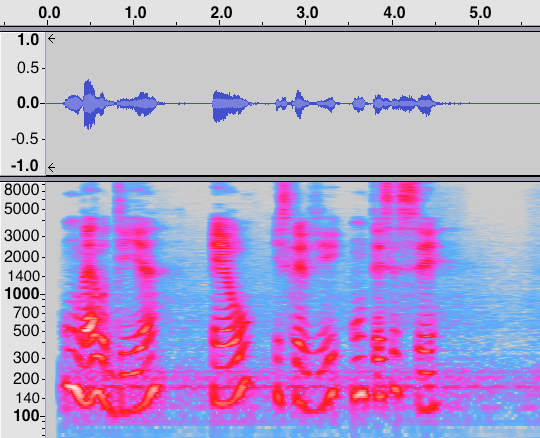
\includegraphics[width=0.5\textwidth]{Imagens/espectro.png}
  \caption[Representações temporal e espectral de uma gravação de voz]{Representações temporal (acima) e espectral (abaixo) de uma gravação de voz. Fonte: própria}
  \label{fig:spectrum}
\end{figure}

% quanto a $ f_0 $, f1, ver Taylor p. 185/161

\subsubsection{Síntese concatenativa}
Devido aos problemas destacados para as outras duas abordagens, a maior parte
dos sistemas TTS, até alguns anos atrás, utilizava síntese concatenativa, que
consiste na gravação de múltiplas frases posteriormente divididas
em fragmentos de granularidade variável, como ilustrado a seguir.

Para vocabulários com poucas palavras, como um sistema de anúncios de um metrô, é
suficiente gravar frases completas e palavras que podem variar dentro da frase.
Ao enunciar ``Este metrô para nas estações Catete, Glória, Cinelândia [...]'',
por exemplo, o fragmento ``Este metrô para nas estações'' pode advir de uma
única gravação, enquanto os nomes individuais das estações são provenientes de
outras gravações, concatenadas. Para obter sistemas TTS mais flexíveis, porém,
as gravações devem ser separadas em unidades menores, como fones ou dífonos --
 pares de fones -- que podem ser então concatenados para formar até mesmo
palavras que não foram gravadas.

Mais recentemente, foi popularizada uma nova classe de algoritmos para
síntese concatenativa denominada \emph{unit selection synthesis}, abordagem
probabilística que funciona através da minimização de duas função de custo, uma
para fones individuais e outra para a junção entre dois fones.
\citeonline{black} argumenta que, com advento desse tipo de síntese, a fala
gerada passou a ser natural o suficiente para ser possivelmente confundida com a de um humano.

\subsection{Síntese por \emph{Hidden Markov Models} e \emph{Deep Neural Networks}}
\label{hmmsynthesis}
\citeonline{zen} descrevem síntese por \emph{Hidden Markov Models} como uma
maneira paramétrica de produzir fala. Nela, um banco de dados com gravações é
utilizado para treinar um modelo a partir de múltiplos parâmetros de entrada
dividos em duas categorias: \emph{excitation parameters} e
\emph{spectral parameters}. Com este método de síntese de fala, há unificação
dos módulos de \emph{front end} e \emph{back end}. Mais recentemente, esse
modelo, denominado \emph{Statistical Parametric Speech Synthesis} foi adaptado
para utilizar redes neurais profundas no lugar de cadeias de Markov
\cite{dnngoogle}. Os resultados mais naturais para síntese de fala até o momento
foram obtidos por este paradigma.

% However, by properly combining these two, we may be able to obtain a first-rate complementary hybrid approach that can solve their respective drawbacks while retaining all their advantages. In the near fu- ture, we may find the holy grail of corpus-based speech synthe- sis fusing statistical parametric and unit-selection synthesi

% Statistical parametric speech synthesis provides a new frame- work for jointly optimizing the front-end (text analysis) and back-end (waveform generation) modules of text-to-speech (TTS) systems. These two modules are conventionally con- structed independently. The text-analysis module is trained us- ing text corpora and often includes statistical models to analyze text, e.g., the phrasing boundary, accent, and POS. The wave- form generation module, on the other hand, is trained using a labeled speech database. In statistical parametric synthesis, this module includes acoustic models. If these two modules are jointly estimated as a unified statistical model, it is expected to improve the overall performance of a TTS system. Based on this idea, Oura et al. proposed an integrated model for linguistic and acoustic modeling and demonstrated its effectiveness (Oura et al., 2008a).
% 
% \subsubsection{Síntese por \emph{Deep Neural Networks}}

% Intonational phrase: sintagmas entoacionais
% Tone boundary: fronteira prosódica?
% Pitch accent: acento de pitch

% https://www.ime.usp.br/~cpaz/downloads/algorithm-portuguese.pdf

% http://hts.sp.nitech.ac.jp/
% Algumas vozes para o MaryTTS \cite{marytts} utilizam HMMs, isto é, Modelos
% ocultos de Markov para \emph{unit selection}. Há, inclusive, uma voz brasileira
% feita a partir de HMMs: \cite{couto}.
% Projetos mais recentes como \cite{merlin,dnngoogle} utilizam redes neurais para
% estimação de parâmetros. O trabalho da Google informa? que a estimação da curva
% $ f_0 $ é uma possível melhoria.

	% Capítulo 3 - Referencial ou embasamento teórico
% Revisão da literatura
% texto no qual se deve apresentar os aspectos teóricos, isto é, os conceitos utilizados e a definição dos mesmos; nesta parte faz-se a revisão de literatura sobre o assunto, resumindo-se os resultados de estudos feitos por outros autores, cujas obras citadas e consultadas devem constar nas referências;

\simb[\% (fronteira de enunciado para ToBI)]
\abrv[INTSINT -- \emph{International Transcription System for Intonation}]
\abrv[HMM -- \emph{Hidden Markov Model}]

\chapter{Revisão da literatura}

% Intonational phrase: sintagmas entoacionais
% Tone boundary: fronteira prosódica?
% Pitch accent: acento de pitch

% https://www.ime.usp.br/~cpaz/downloads/algorithm-portuguese.pdf

\subsection{Abordagens}
\subsubsection{Klaat}
Síntese por formantes. \cite{espeakng} usa uma mistura do algoritmo de Klatt com
sons de consoantes pré-gravados.
\subsubsection{Unit selection e dífonos}
Abordagem utilizada pelo programa MBROLA. Consiste em gravar fala, separar
pedaços de dois em dois.

Algumas vozes para o MaryTTS \cite{marytts} utilizam HMMs, isto é, Modelos
ocultos de Markov para \emph{unit selection}. Há, inclusive, uma voz brasileira
feita a partir de HMMs: \cite{couto}.
\subsubsection{DNN}

% Resultados realistas, mas não há como controlar parâmetros: \cite{merlin}

\section{Sistemas TTS}
\subsubsection{MBROLA}
Três vozes

\section{Sistemas TTS com suporte a português}
\subsection{MaryTTS}
Projeto FalaBrasil \cite{falabrasil}, \cite{couto}
\subsubsection{G2P}
Para o português brasileiro, foram encontrados os conversores
da USP: \cite{g2pusp} do projeto falabrasil: \cite{falabrasil}.
\subsection{LianeTTS}
Projeto da SERPRO LianeTTS (MBROLA)
\subsection{espeak}
Projeto do Dunn

\subsection{Prosódia no português brasileiro}
Trabalhos de Moraes, Tenani, ...
\subsection{Modelos de prosódia}
\subsubsection{Modelo autossegmental e métrico}
Modelo autossegmental e métrico: Pierrehumbert, Moraes (pitch analysis by synthesis).
ref Moraes, Intonation Systems (20 languages).
\subsubsection{IPO}
% página 32
\cite{ipo} analisa a prosódia para o português brasileiro através do modelo IPO,
seguindo crítica de Lucente que o sistema ToBI é inapropriado.
 % "esse sistema de notação não abarca certas características fonéticas das curvas de F0 que perceptivamente são relevantes para o reconhecimento desses contornos"
\subsubsection{INTSINT}
INTSINT é um sistema de anotação para prosódia.
% The AM model is phonological, the INTSINT model phonetic and the Fujisaki and Tilt models acoustic''
	% Capítulo 4 - Metodologia
% Implementação
% deve constar o instrumental, os métodos e as técnicas aplicados para a elaboração do trabalho;

\abrv[MBRPSOLA -- Multi-Band Resynthesis Pitch Synchronous Overlap and Add]
\simb[ms (milissegundos)]
\simb[Hz (Hertz)]
\chapter{Editor de prosódia}

\section{Implementação}

\subsection{espeak-ng}
Foi utilizado o programa \emph{open-source} espeak-ng \cite{espeakng} para realizar a normalização de texto e realizar a conversão grafema-fonema, ou seja, obter a partir do texto de entrada uma representação em fonemas. O resultado é passado para o programa desenvolvido neste trabalho.

Apesar da existência de outras ferramentas para \emph{front-end} para o português brasileiro, optamos por esta pela facilidade de instalação, marcação de ênfase disponível, etc.

\subsection{MBROLA}
Baseado no algoritmo {MBRPSOLA} \cite{mbrpsola}. É um \emph{back-end}. O programa recebe uma lista de fones. Um exemplo de entrada é:

\begin{lstlisting}
      _ 150 50 150
      o 108 50 125
      l 125 50 75
      a 116 20 232 80 300
      _ 150 50 150
\end{lstlisting}

\subsubsection{Formato}
Em cada linha, tem-se um fone ou um silêncio representado pelo \emph{underscore} seguido por uma duração em milissegundos e, por último, um ou mais pares de porcentagem e frequência em Hertz determinando alvos para a curva F0. Como exemplo, na quarta linha temos o fone \/a\/ com duração de 116 ms e dois alvos para altura, 232 Hz em 20\% e 300 Hz em 80\%.

% referência?
Cada voz gravada provê uma tabela com os fones que podem ser utilizados. Utilizamos neste trabalho a voz br3 desenvolvida por Denis R. Costa disponível no site oficial do projeto MBROLA.

\subsection{Arquitetura}
Diagrama aqui

\subsection{Módulo de prosódia}

\subsection{Editor gráfico}
O programa foi codificado em Python em sua versão 3.6. Pega resultado do espeak-ng, processa com editor gráfico e gera MBROLA.

Para alterar a prosódia manualmente, foi desenvolvido um editor gráfico
para \emph{web} utilizando HTML, CSS e JavaScript. A duração e altura de cada
fone pode ser especificado arrastando barras de controle. O editor se comunica
com o espeak-ng e MBROLA através de um servidor programado em Python utilizando
o \emph{framework} Flask para prover \emph{endpoints} de uma API REST.

\begin{figure}[!htbp]
\centering
\scalebox{0.65}{
    \begin{tikzpicture}[auto, >={Latex[inset=0pt, length=3mm, angle'=28,round]}, box/.style={draw,rounded corners,text width=3.0cm,align=center}]
    \node[] (txt) {Texto};
    \node[box, right=of txt] (esp)
        {espeak-ng};
    \node[box, right=of esp] (con)
        {espeak para MBROLA};
    \node[box, right=of con] (mbr)
        {MBROLA};

    \node[box, below=of con] (ser)
        {Servidor};
        
    \draw[->] (txt) -- (esp);

    \end{tikzpicture}
}
\caption{Arquitetura do sistema desenvolvido}
\label{fig:lol}
\end{figure}



% \begin{figure}[!htbp]
% \centering
% \scalebox{0.65}{
%     \begin{tikzpicture}[auto, >={Latex[inset=0pt, length=3mm, angle'=28,round]}, box/.style={draw,rounded corners,text width=3.0cm,align=center}]
%     \node[] (txt) {Texto};
%     \node[box, right=0.7cm of txt] (pre)
%         {Pré-processador};
%     \node[box, right=0.2cm of pre] (mor)
%         {Analisador morfológico};
%     \node[box, right=0.2cm of mor] (con)
%         {Analisador de contexto};
%     \node[box, right=of con] (let)
%         {Módulo letra-som};
%     \node[box, right=of let] (pro)
%         {Gerador de prosódia};
%         
%     \draw[->] (txt) -- (pre);
%         
%     \node[box, fit=(pre)(mor)(con), label={[name=morfos_l] Analisador morfossintático}] (morfos) {};
%     \node[box, fit=(let)] (letsom) {};
%     \node[box, fit=(pro)] (proger) {};
%     
%     \node[inner sep=0, fit=(morfos)(letsom)(proger)] (all) {};
%     \node[box,
%           inner sep=0,
%           yshift=-0.75cm,
%           fit=(morfos.west)(proger.east),
%           label=center:Estrutura de dados,
%           minimum height=1cm,
%           below of=all]
%         (dad) {};
%     
%     \node[box, fit=(morfos)(morfos_l)(letsom)(proger)(dad), label=Processamento de linguagem natural] (nlp) {};
%     
%     \node[right=of dad, align=left] (out) {\emph{phones}\\ prosódia};
%     
%     \draw[->] (pre) -- (pre |- dad.north);
%     \draw[<->] (mor) -- (mor |- dad.north);
%     \draw[<->] (con) -- (con |- dad.north);
%     \draw[<->] (let) -- (let |- dad.north);
%     \draw[<->] (pro) -- (pro |- dad.north);
%     
%     \draw[->] (dad) -- (out);
%         
%     \end{tikzpicture}
% }
% \caption{Arquitetura de um sistema de geração de prosódia}
% \label{fig:nlpdiagram}
% \end{figure}

	% Capítulo 5 - Resultados
% devem ser apresentados, de forma objetiva, precisa e clara, tanto os resultados positivos quanto os negativos que foram obtidos com o desenvolvimento do trabalho, sendo feita uma discussão que consiste na avaliação circunstanciada, na qual se estabelecem relações, deduções e generalizações.

\chapter{Resultados}
Com o levantamento dos sistemas TTS desenvolvidos para o português brasileiro, é
possível observar que há carência de suporte à síntese emocional e expressiva.
Seguindo o modelo de funções prosódicas de \cite{taylor2009}, os sistemas
estudados concentram-se na geração de prosódia suprassegmental, mas não há
suporte algum à geração de prosódia afetiva e aumentativa atualmente.

Linguagens de marcação como SSML e EmotionML já começaram a ser integradas a
\emph{frameworks open-source} e sistemas comerciais de TTS para múltiplas
línguas, mas não foram encontrados trabalhos para o português brasileiro.

Estudando os modelos de anotação entoacional, percebe-se que ainda não há uma
solução considerada mais apropriada para analisar o português brasileiro. Há,
por outro lado, uma grande quantidade de trabalhos de análise de contornos
melódicos que podem ser futuramente adaptados a sistemas TTS expressivos,
servindo como base para a geração manual ou automática de prosódia afetiva.

Encontramos lacunas que precisam ser preenchidas, como a criação de corpus
anotados prosodicamente e algoritmos de compreensão textual para geração de
anotações.

Com o desenvolvimento de programas para linha de comandos e para \emph{desktop}
neste trabalho, dá-se um passo inicial para a melhoria de prosódia afetiva e
aumentativa em sistemas TTS para o português brasileiro.
	% Considerações finais
% As considerações finais formam a parte final (fechamento) do texto, sendo dito de forma resumida (1) o que foi desenvolvido no presente trabalho e quais os resultados do mesmo, (2) o que se pôde concluir após o desenvolvimento bem como as principais contribuições do trabalho, e (3) perspectivas para o desenvolvimento de trabalhos futuros. O texto referente às considerações finais do autor deve salientar a extensão e os resultados da contribuição do trabalho e os argumentos utilizados estar baseados em dados comprovados e fundamentados nos resultados e na discussão do texto, contendo deduções lógicas correspondentes aos objetivos do trabalho, propostos inicialmente.

\chapter{Considerações finais}
Neste trabalho foi apresentada a definição de um sistema TTS, bem como a descrição
de seus componentes principais e possíveis implementações para cada módulo.
Também foi realizada uma busca dos sistemas TTS \emph{open-source} e comerciais
existentes. Com o objetivo de melhorar a geração de prosódia, foi feita uma
revisão de prosódia na linguística, descrevendo os principais sistemas de
anotação usados na fonologia entoacional, principalmente aplicados ao português
brasileiro. Investigamos como a prosódia funciona nos sistemas encontrados e
identificamos que, enquanto a geração de prosódia suprassegmental em trabalhos
recentes já produz resultados satisfatórios, ainda há desafios quando à síntese
de fala expressiva relacionada à prosódia afetiva e aumentativa.

\section{Trabalhos futuros}
Foi identificado que ainda há um significante desafio para a geração de prosódia
afetiva automática a partir de um texto não anotado. Possíveis soluções para
avanço nesta área incluem:
\begin{itemize}
\item Expansão do sistema desenvolvido neste trabalho para adicionar suporte a
  mais modelos notação entoacional.
\item Avaliação estatística da qualidade de falas geradas com a aplicação desenvolvida comparada a outros sistemas \emph{open-source} e comerciais
\item Adicionar suporte a SSML e EmotionML ao sistema desenvolvido, gerando
  curvas F0 a partir de linguagens de marcação
\item Uso técnicas de técnicas de \emph{Natural Language Understanding} para gerar notação EmotionML automaticamente.
\item Desenvolvimento de corpus anotados com prosódia para o português brasileiro.
\end{itemize}

% Usar técnicas de Natural Language Understanding para gerar prosódia utilizando notação desenvolvida neste trabalho
% corpus anotados para o português
% https://corplinguistics.wordpress.com/2012/03/08/prosodically-annotated-corpora/
	
	% Bibliografia (arquivo Capitulos/Referencias.bib)
	\bibliography{Capitulos/Referencias}
	\bibliographystyle{abnt-alf}
	
	% % Apêndice A (arquivo Includes/ApendiceA)
	% Apêndice
\apendice
\chapter{Primeiro apêndice}

\begin{figure}
  \centering
    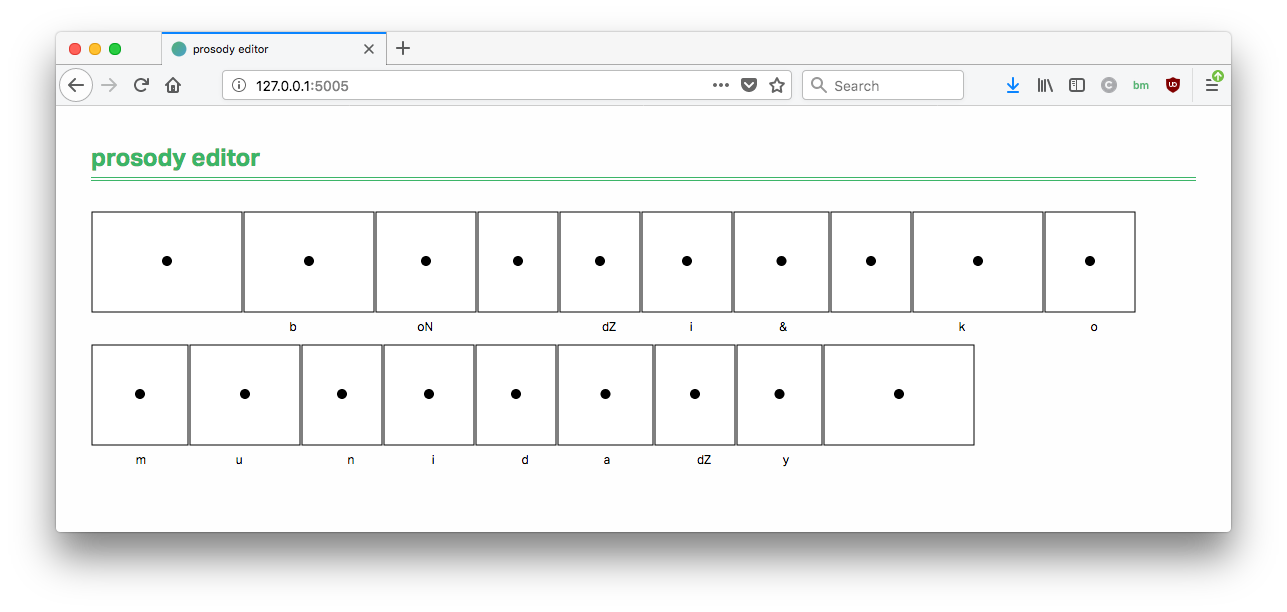
\includegraphics[width=1\textwidth]{Imagens/editor.png}
  \caption{Editor gráfico}
\end{figure}

\begin{lstlisting}[caption=Servidor, label=servidor, language=Python]
import sqlite3
import sampa_mbrola
from flask import Flask, g, jsonify, render_template, abort, request
from flask_cors import CORS

app = Flask(__name__)
CORS(app)

@app.route('/api/espeak', methods=['POST'])
def frontend():
    text = request.form['text']
    converter = sampa_mbrola.Converter()
    sentence = converter.convert_sentence(text)
    return jsonify(sentence.dictify())

@app.route('/api/mbrola', methods=['GET'])
def mbrola(page):
    pass

if __name__ == '__main__':
    app.run(debug=True)
\end{lstlisting}

\begin{lstlisting}[caption=Conversor eSpeakNG-MBROLA, label=conversao, language=Python]
import sys
import re
import subprocess
import random
import json
from collections import OrderedDict
from typing import List

def flatten(lst: list):
    return [item for sublist in lst for item in sublist]

class Phone():
    def __init__(
            self,
            phone_sampa: str,
            phone_mbrola: str,
            duration: int,
            pitch_changes: list
    ):
        self.phone_sampa = phone_sampa
        self.phone_mbrola = phone_mbrola
        self.duration = duration
        self.pitch_changes = pitch_changes

    def as_line(self):
        return "{} {} {}".format(
            self.phone_mbrola,
            self.duration,
            " ".join([str(item) for item in flatten(self.pitch_changes)])
        )

class Sentence():
    def __init__(self, phones: List[Phone]=None):
        if phones is None:
            self.phones = []
        else:
            self.phones = phones

    def mbrola_phones(self):
        return [phone.phone_mbrola for phone in self.phones]

    def dictify(self):
        return [vars(phone) for phone in self.phones]

    def __repr__(self):
        return "\n".join([phone.as_line() for phone in self.phones])


class Converter():
    def __init__(self):
        self.load_sampa_mbrola()
        self.load_durations()

    def load_sampa_mbrola(self):
        equivs = {}
        with open("sampa_mbrola.tbl") as f:
            for line in f:
                k, v, _ = line.split()
                equivs[k] = v

        self.equivs = OrderedDict(
            sorted(equivs.items(), key=lambda t: -len(t[0])))

    def load_durations(self):
        durations = {}
        with open("durations.tbl") as f:
            for line in f:
                k, v = line.split()
                durations[k] = v

        self.durations = durations

    def convert_phoneme(self, sentence: str) -> tuple:
        """Returns first phone from the sentence"""

        if sentence[0] == " ":
            return ("_", 1)
        elif self.equivs:
            # s is a special case, needs to peek next
            if sentence[0] == "s":
                if sentence[1] in "aeiou&":
                    return ("s", 1)

            for equiv in self.equivs.items():

                if re.match(re.escape(equiv[0]), sentence):
                    # print("match:", equiv[0], phoneme, "=", equiv[1])
                    return (equiv[1], len(equiv[0]))

        # print("didn't match", phoneme)
        return (phoneme[0], 1)

    def get_duration(self, phoneme: str) -> int:
        if self.durations and phoneme in self.durations:
            return self.durations[phoneme]
        else:
            return 100

    def convert_sentence(self, input_str: str) -> Sentence:
        sentence = Sentence()
        sentence.phones.append(Phone(" ", "_", 150, [[50, 150]]))

        ignored = ["@", "\n", ",", "'", "^", ";"]

        sampa = self.text_to_sampa(input_str)
        sampa = sampa.replace("'", "")
        print(";; ", sampa)

        while sampa:
            if sampa[0] not in ignored:
                converted = self.convert_phoneme(sampa)
                phone_sampa = sampa[:converted[1]]
                sampa = sampa[converted[1]:]

                duration = self.get_duration(converted[0])
                phone = Phone(
                    phone_sampa = phone_sampa,
                    phone_mbrola = converted[0],
                    duration = int(duration),
                    pitch_changes = [[50, 150]] # percentage, Hz
                )

                sentence.phones.append(phone)
            else:
                sampa = sampa[1:]

        sentence.phones.append(Phone(" ", "_", 150, [[50, 150]]))
        return sentence

    def text_to_sampa(self, sentence: str) -> str:
        espeak_str = "espeak-ng -v pt-br '{}' -x -q".format(sentence)

        p = subprocess.Popen(espeak_str, stdout=subprocess.PIPE, shell=True)
        (output, err) = p.communicate()
        p_status = p.wait()
        output = output.decode("utf-8")
        output = output.replace("\n", "").strip()
        return output


if __name__ == "__main__":
    converter = Converter()

    for line in sys.stdin:
        print(";;", line)
        print(converter.convert_sentence(line))
\end{lstlisting}

\begin{lstlisting}[caption=Editor gráfico, label=editorjs, language=Python]
var app = new Vue({
  el: '#app',
  data: {
    phones: [],
    height: 300
  },
  mounted: function() {
    var self = this;
    const requestURL = "http://127.0.0.1:5000/api/espeak";
    let XHR = new XMLHttpRequest();
    let FD  = new FormData();

    FD.append("text", "Bom dia, comunidade");

    XHR.open("POST", requestURL);
    XHR.send(FD);

    XHR.onreadystatechange = function() {
      if (XHR.readyState === XMLHttpRequest.DONE) {
        if (XHR.status === 200) {
          const results = JSON.parse(XHR.responseText);
          self.phones = results;
        }
      }
    };
  },
  computed: {
    totalDuration: function() {
      let durations = this.phones.map((phone) => phone.duration);
      console.log(durations.reduce((acc, val) => acc + val, 0));
      return durations.reduce((acc, val) => acc + val, 0);
    }
  }
});
\end{lstlisting}

\begin{lstlisting}[caption=Exemplo de resposta para \emph{endpoint} do eSpeakNG, label=espeakpost, language=Python]
[
  {
    "duration": 150,
    "phone_mbrola": "_",
    "phone_sampa": " ",
    "pitch_changes": [[50, 150]
    ]
  },
  {
    "duration": 80,
    "phone_mbrola": "n",
    "phone_sampa": "n",
    "pitch_changes": [[50, 150]]
  },
  {
    "duration": 110,
    "phone_mbrola": "u",
    "phone_sampa": "U",
    "pitch_changes": [[50, 150]]
  },
  ...
  {
    "duration": 150,
    "phone_mbrola": "_",
    "phone_sampa": " ",
    "pitch_changes": [[50, 150]]
  }
]
\end{lstlisting}

\begin{lstlisting}[caption=Exemplo de resposta para \emph{endpoint} do MBROLA, label=mbrolaget, language=Python]
{
  "mp3_file": "07acc5c4ba924294.mp3"
}
\end{lstlisting}

\begin{lstlisting}[caption=Gerador de f0 a partir do modelo INTSINT, label=intsintpy, language=Python]
import json

def get_duration(self, phoneme: str) -> int:
    if self.durations and phoneme in self.durations:
        return self.durations[phoneme]
    else:
        return 100

def convert_sentence(self, input_str: str) -> Sentence:
    sentence = Sentence()
    sentence.phones.append(Phone(" ", "_", 150, [[50, 150]]))

    ignored = ["@", "\n", ",", "'", "^", ";"]

    sampa = self.text_to_sampa(input_str)
    sampa = sampa.replace("'", "")
    print(";; ", sampa)

    while sampa:
        if sampa[0] not in ignored:
            converted = self.convert_phoneme(sampa)
            phone_sampa = sampa[:converted[1]]
            sampa = sampa[converted[1]:]

            duration = self.get_duration(converted[0])
            phone = Phone(
                phone_sampa = phone_sampa,
                phone_mbrola = converted[0],
                duration = int(duration),
                pitch_changes = [[50, 150]] # percentage, Hz
            )

            sentence.phones.append(phone)
        else:
            sampa = sampa[1:]

    sentence.phones.append(Phone(" ", "_", 150, [[50, 150]]))
    return sentence

def text_to_sampa(self, sentence: str) -> str:
    espeak_str = "espeak-ng -v pt-br '{}' -x -q".format(sentence)

    p = subprocess.Popen(espeak_str, stdout=subprocess.PIPE, shell=True)
    (output, err) = p.communicate()
    p_status = p.wait()
    output = output.decode("utf-8")
    output = output.replace("\n", "").strip()
    return output
\end{lstlisting}

	% 
	% % Anexo A (arquivo Includes/AnexoA)
	% % Anexo
\anexo
\chapter{Primeiro anexo}

Os anexos são textos ou documentos não elaborado pelo autor, que servem de fundamentação, comprovação e ilustração.

	
	% Página em branco
	\newpage

\end{document}
